\documentclass[aspectratio=169,UTF8,fontset=windows]{ctexbeamer}

\usetheme{Madrid}
\usecolortheme{default}
\usefonttheme{professionalfonts}

\usepackage{booktabs}
\usepackage{tabularx}
\usepackage{tikz}
\usepackage{xcolor}
\usepackage{array}
\usepackage{listings}
\usetikzlibrary{positioning}

\definecolor{AgentBlue}{HTML}{0B3D5C}
\definecolor{AgentTeal}{HTML}{168A8A}
\definecolor{AgentAmber}{HTML}{D88A24}
\definecolor{AgentInk}{HTML}{1F2933}
\definecolor{AgentGray}{HTML}{E8EEF2}
\definecolor{AgentGreen}{HTML}{2E7D32}
\definecolor{AgentRed}{HTML}{B3261E}

\setbeamercolor{normal text}{fg=AgentInk,bg=white}
\setbeamercolor{structure}{fg=AgentBlue}
\setbeamercolor{frametitle}{fg=white,bg=AgentBlue}
\setbeamercolor{title}{fg=white,bg=AgentBlue}
\setbeamercolor{block title}{fg=white,bg=AgentTeal}
\setbeamercolor{block body}{fg=AgentInk,bg=AgentGray!45}
\setbeamercolor{alerted text}{fg=AgentAmber}
\setbeamertemplate{navigation symbols}{}
\setbeamertemplate{footline}[frame number]

\lstdefinestyle{cmd}{
  basicstyle=\ttfamily\scriptsize,
  backgroundcolor=\color{AgentGray!45},
  frame=single,
  rulecolor=\color{AgentGray},
  breaklines=true,
  columns=fullflexible
}

% Update these macros when a new full Test262 report is available.
\newcommand{\ProjectName}{AgentJS}
\newcommand{\ReportDate}{2026-06-28}
\newcommand{\FullTotal}{53,379}
\newcommand{\FullPassed}{35,472}
\newcommand{\FullFailed}{17,905}
\newcommand{\FullSkipped}{2}
\newcommand{\FullPassRate}{66.45\%}
\newcommand{\FullElapsed}{644.92s}
\newcommand{\FullEvidence}{reports/.test262/test262-full-output/test262-fixRTLE-output.txt}

\newcommand{\progressbar}[2]{%
  \begin{tikzpicture}[baseline=-0.6ex]
    \fill[AgentGray] (0,0) rectangle (5.2,0.22);
    \fill[#2] (0,0) rectangle ({5.2*#1/100},0.22);
  \end{tikzpicture}%
}

\newcommand{\metriccard}[3]{%
  \begin{block}{#1}
    \centering
    {\Large\bfseries #2}\\[-0.2em]
    {\scriptsize #3}
  \end{block}
}

\newcommand{\leadtext}[1]{%
  {\large\bfseries #1}\par\vspace{0.35em}
}

\newcommand{\smallsource}[1]{%
  {\tiny\color{AgentInk!70}#1}
}

\title[\ProjectName{} 工作流与成果]{\ProjectName{}：面向智能体负载的轻量 JavaScript 引擎}
\subtitle{工作流程、工程成果与 Test262 通过率}
\author{OS 功能赛项目组}
\institute{Rust native backend}
\date{\ReportDate}

\begin{document}

\begin{frame}
  \titlepage
\end{frame}

\begin{frame}{汇报主线}
  \leadtext{从“能跑 JavaScript”到“可验证的轻量执行引擎”。}

  \ProjectName{} 的目标场景是 AI agent 中短生命周期、高频率的小段
  JavaScript 执行。我们的路线不是把现有引擎包一层命令行，而是在 Rust 中
  逐步替换 JS 执行链路，并用 Test262、版本门禁和失败簇修复工作流驱动收敛。

  \vspace{0.8em}
  \begin{tabularx}{\textwidth}{>{\bfseries}p{0.16\textwidth} X >{\raggedleft\arraybackslash}p{0.25\textwidth}}
    \toprule
    目标 & 轻量、跨平台、资源可控 & 短任务优先 \\
    方法 & native lexer / parser / bytecode / VM / runtime / builtins & 自研主链路 \\
    结果 & 全量 Test262 当前可见记录超过 60\% & {\Large\bfseries \FullPassRate} \\
    \bottomrule
  \end{tabularx}
\end{frame}

\begin{frame}{问题背景与目标}
  在 agent 场景里，JavaScript 往往不是一个长期驻留的浏览器页面，而是一段
  需要立刻执行、立刻返回结果的工具脚本。浏览器级引擎覆盖面很完整，但它的
  工程形态未必总是适合短任务、高频调用和强资源边界的场景。

  \vspace{0.6em}
  因此我们把目标收束为四件事：用 Rust 实现轻量级 JS 执行引擎；默认走
  native backend；二进制可在 Linux、macOS、Windows 上运行；并用
  ECMAScript Test262 的通过率证明标准兼容度。

  \vspace{0.8em}
  \begin{tabularx}{\textwidth}{>{\bfseries}p{0.22\textwidth} X}
    \toprule
    评价维度 & 我们的对应材料 \\
    \midrule
    文档完整度 & 架构、接口、版本流程、fixup 流程和测试报告 \\
    功能测试 & Test262 full suite、focused scan、固定回归门 \\
    性能 benchmark & cold / warm / cached microbenchmark 与 JetStream adapter \\
    创新性 & agent 场景、可控 host surface、crash-safe dashboard \\
    \bottomrule
  \end{tabularx}
\end{frame}

\begin{frame}{设计原则：轻量与可控}
  \leadtext{目标不是“大而全”，而是“足够标准、足够快、足够安全”。}

  轻量主要体现在依赖边界和 host surface 上：标准构建默认选择 native
  backend，Boa 和 QuickJS 只作为显式参考；运行环境只暴露必要输出和
  Test262 host 支持，不把文件系统、进程、网络等能力直接交给脚本。

  \vspace{0.5em}
  高效主要体现在执行形态上：source 会被解析、编译为字节码，再交给 VM 和
  runtime；相关调用可以复用 runtime 状态；重复脚本可以命中 per-isolate
  缓存，减少重复 parse/compile 的成本。

  \vspace{0.6em}
  \begin{center}
    \progressbar{100}{AgentTeal}\hspace{0.8em}
    {\small 资源预算覆盖循环、递归、VM 栈、堆对象、堆字节和墙钟时间。}
  \end{center}
\end{frame}

\begin{frame}{Native 执行链路}
  \begin{center}
  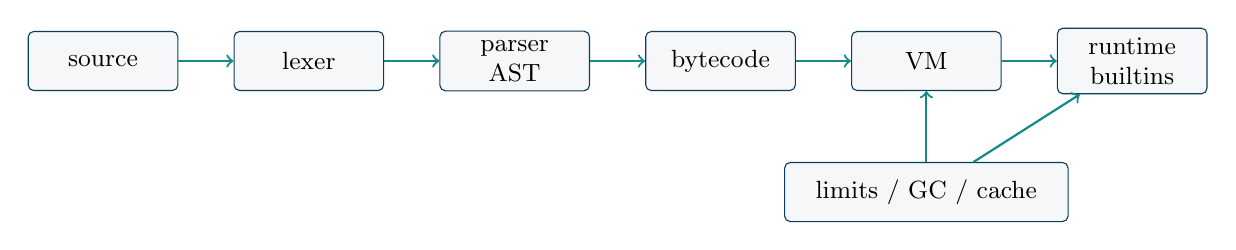
\begin{tikzpicture}[
    node distance=0.7cm,
    stage/.style={draw=AgentBlue, fill=AgentGray!45, rounded corners=2pt,
      minimum width=1.9cm, minimum height=0.75cm, align=center, font=\small},
    arrow/.style={->, thick, color=AgentTeal}
  ]
    \node[stage] (source) {source};
    \node[stage, right=of source] (lexer) {lexer};
    \node[stage, right=of lexer] (parser) {parser\\AST};
    \node[stage, right=of parser] (bc) {bytecode};
    \node[stage, right=of bc] (vm) {VM};
    \node[stage, right=of vm] (rt) {runtime\\builtins};
    \draw[arrow] (source) -- (lexer);
    \draw[arrow] (lexer) -- (parser);
    \draw[arrow] (parser) -- (bc);
    \draw[arrow] (bc) -- (vm);
    \draw[arrow] (vm) -- (rt);
    \node[stage, below=0.9cm of vm, minimum width=3.6cm] (guard) {limits / GC / cache};
    \draw[arrow] (guard) -- (vm);
    \draw[arrow] (guard) -- (rt);
  \end{tikzpicture}
  \end{center}

  \vspace{0.5em}
  \textbf{边界说明：}
  \texttt{contracts.rs} 冻结 SourceParser、ProgramCompiler、ChunkExecutor、
  NativePipeline 等协作接口；\texttt{backend/native.rs} 负责装配，不承载
  具体语言实现。这样前端、编译器、VM/runtime 可以并行推进，也便于单独测试。
\end{frame}

\begin{frame}{模块分工与协作接口}
  \begin{tabularx}{\textwidth}{>{\bfseries}p{0.18\textwidth} X X}
    \toprule
    Track & 负责范围 & 独立验证方式 \\
    \midrule
    A 前端 & \texttt{lexer/}、\texttt{ast/}、\texttt{parser/} & source/token 到 AST \\
    B 编译器 & \texttt{bytecode/} & 手工 AST 到 Chunk \\
    C 执行内核 & \texttt{vm/}、\texttt{runtime/}、\texttt{builtins/} & 手工 Chunk 或 Runtime API \\
    D 集成 & \texttt{backend/}、CLI、Test262、CI、报告 & source 到 native 执行结果 \\
    \bottomrule
  \end{tabularx}

  \vspace{0.8em}
  协作上的关键做法是把“接口稳定”和“实现并行”拆开：共享 AST、Opcode、
  Runtime API 先冻结，未完成的上下游用 fake stage 或手工 AST/Chunk 隔离。
  Boa 只作差分参考，不作为 native 通过率的一部分。
\end{frame}

\begin{frame}{从版本开发到 Fixup 冲刺}
  前期的 Native V1-V11 按语言能力和运行时基础设施推进。每个版本都有
  scope、interface、team plan 和 scan manifest，固定 Test262 门禁用于保证
  旧能力不回退。

  \vspace{0.6em}
  当主链路已经成型后，项目进入 Fixup 冲刺：分工不再按 parser/compiler/runtime
  分层，而是按高收益失败簇闭环，例如 Builtins/Temporal/Descriptor、
  RegExp/String dispatch、Language/Module/Async Protocol。这样每个 track 都能
  对“新增多少 passed、是否引入回归”负责。

  \vspace{0.4em}
  \begin{center}
    {\small baseline \(\rightarrow\) focused fix \(\rightarrow\) regression gate \(\rightarrow\) full scan \(\rightarrow\) report}
  \end{center}
\end{frame}

\begin{frame}{测试体系}
  测试分成两层。第一层是工程质量门，保证代码能稳定合入：
  \texttt{cargo fmt}、\texttt{cargo check}、\texttt{cargo test}、
  \texttt{cargo clippy} 和 native contract tests。

  \vspace{0.7em}
  第二层是 Test262 门。固定版本门验证已完成能力不回退；5,000-case scan
  跟踪版本或 fixup 阶段的收益；full suite 使用 \FullTotal{} 条用例做正式
  通过率展示。skipped、timeout、crash 都被单独记录，不计入 passed。

  \vspace{0.8em}
  \begin{tabularx}{\textwidth}{>{\bfseries}p{0.24\textwidth} X}
    \toprule
    fixed gate & 小而严格，防回归 \\
    focused scan & 中等规模，看收益和失败簇 \\
    full suite & 最终口径，展示整体通过率 \\
    \bottomrule
  \end{tabularx}
\end{frame}

\begin{frame}{全量 Test262 成果}
  \begin{columns}[T,onlytextwidth]
    \column{0.42\textwidth}
      {\Huge\bfseries \FullPassRate}\par
      \vspace{0.3em}
      {\large \FullPassed{} / \FullTotal{} passed}\par
      \vspace{0.6em}
      当前可见 full-output 记录已经越过 60\% 目标线，并且 skipped 只有
      \FullSkipped{} 条，不混入 passed 统计。
    \column{0.53\textwidth}
      \begin{tabularx}{\textwidth}{>{\bfseries}l X}
        \toprule
        Total & \FullTotal \\
        Passed & \FullPassed \\
        Failed & \FullFailed \\
        Skipped & \FullSkipped \\
        Elapsed & \FullElapsed \\
        \bottomrule
      \end{tabularx}
      \vspace{0.4em}
      \progressbar{66.45}{AgentGreen}\hspace{0.6em}{\small 超过 60\% 目标线}
  \end{columns}

  \vspace{0.5em}
  \smallsource{数据来源：\texttt{\FullEvidence{}}}
\end{frame}

\begin{frame}{通过率演进}
  \begin{tabularx}{\textwidth}{>{\bfseries}p{0.22\textwidth} r r r X}
    \toprule
    阶段记录 & Passed & Failed & Pass rate & 说明 \\
    \midrule
    fixbug4 & 28,468 & 24,909 & 53.33\% & 进入功能簇修复后的中期结果 \\
    fixbug5 & 32,097 & 21,280 & 60.13\% & 首次越过 60\% 目标线 \\
    fixbug6 & 34,640 & 18,737 & 64.89\% & 持续收割高收益失败簇 \\
    fixRTLE & 35,472 & 17,905 & 66.45\% & 当前框架采用的展示数据 \\
    \bottomrule
  \end{tabularx}

  \vspace{0.8em}
  \begin{center}
    \progressbar{53.33}{AgentAmber}\quad
    \progressbar{60.13}{AgentTeal}\quad
    \progressbar{64.89}{AgentTeal}\quad
    \progressbar{66.45}{AgentGreen}
  \end{center}
\end{frame}

\begin{frame}{重点能力域快照}
  \begin{tabularx}{\textwidth}{>{\bfseries}p{0.24\textwidth} r r r X}
    \toprule
    能力域 & Total & Passed & Rate & 证据文件 \\
    \midrule
    Object & 3,411 & 3,133 & 91.85\% & \texttt{fix8-p1-object-final.json} \\
    Array & 3,081 & 2,366 & 76.79\% & \texttt{fix8-p1-array-final.json} \\
    V6 core scan & 2,199 & 1,832 & 83.31\% & \texttt{native-v6-frontend-summary.json} \\
    RegExp focused & 1,879 & 1,162 & 61.84\% & \texttt{post-fix2-c-final-regexp.json} \\
    V7 diagnostic gate & 3,034 & 1,973 & 65.03\% & \texttt{native-v7-verbose.txt} \\
    \bottomrule
  \end{tabularx}

  \vspace{0.4em}
  {\small 这些不是全量通过率，而是说明关键功能簇已经具备可答辩的成熟度证据。}
\end{frame}

\begin{frame}{性能与轻量化证据}
  性能部分目前更适合作为“可复现实验框架”展示：release native binary 已经
  能跑 microbenchmark，命令会区分 cold isolate、warm runtime 和 warm cached
  runtime；JetStream 2 CLI adapter 也已经建立，并保留 Node/V8 control 来证明
  生成 workload 和评分流程本身是可用的。

  \vspace{0.7em}
  答辩时建议把这一页和下一页连起来讲：我们已经把性能测量路径铺好，后续只要
  补入同机数据，就能形成“轻量引擎在短任务上的成本曲线”。

  \vspace{0.8em}
  \begin{tabularx}{\textwidth}{>{\bfseries}p{0.22\textwidth} X}
    \toprule
    已有证据 & release binary、bench 命令、JetStream adapter、crash-safe dashboard \\
    待补数字 & binary size、cold latency、warm cached latency、peak memory、对照引擎 \\
    \bottomrule
  \end{tabularx}
\end{frame}

\begin{frame}[fragile]{可复现实验命令}
  \begin{lstlisting}[style=cmd]
cargo build --release --no-default-features

cargo run --release --no-default-features -- test262 \
  --backend native --root test262 --suite test --jobs 4 --progress

cargo run --release --no-default-features -- bench 1000

.\scripts\run-jetstream2.ps1 -Tests richards,splay -Iterations 5
  \end{lstlisting}

  \vspace{0.4em}
  \textbf{报告原则：}
  跳过、超时、崩溃和未捕获记录不计入通过；Native 与 Boa、Node/V8、QuickJS
  结果分开报告，避免把参考引擎能力混入自研路径。
\end{frame}

\begin{frame}{创新点}
  \leadtext{创新点不是某一个孤立功能，而是工程取向的组合。}

  第一，Agent 场景优先。fresh isolate 适合彼此独立的工具调用，可复用 runtime
  适合 REPL 或连续会话，脚本缓存则服务于高频重复执行。

  \vspace{0.45em}
  第二，可审计工作流。每个版本和 fixup 阶段都有 baseline、scan、报告和门禁；
  通过率的变化能追溯到具体失败簇和具体修复。

  \vspace{0.45em}
  第三，故障隔离。Test262 dashboard 对 crash、timeout、skip 单独分类，既保护
  长时间扫描的稳定性，也避免制造假通过。
\end{frame}

\begin{frame}{当前边界与下一步}
  当前 \FullPassRate{} 说明主链路和大量内建能力已经成型，但剩余失败仍然集中在
  一些“大块能力”上：class/destructuring、module/dynamic import、
  Promise/Iterator、Temporal/Intl，以及 RegExp property escapes 和
  String-RegExp dispatch。

  \vspace{0.7em}
  下一步适合继续沿 Fixup 工作流推进：先锁定最新 full baseline，再按失败簇分配
  track，focused test 看局部收益，fixup scan 看回归，最后用 full Test262 确认
  全局净收益。阶段目标可以自然设为 70\%，同时补齐 cold/warm/cache 的性能报告。

  \vspace{0.8em}
  \begin{tabularx}{\textwidth}{>{\bfseries}p{0.20\textwidth} X}
    \toprule
    技术收敛 & class / module / async / iterator / Temporal / RegExp \\
    数据收敛 & full baseline、fixup scan、性能对照、回归门 \\
    \bottomrule
  \end{tabularx}
\end{frame}

\begin{frame}{总结}
  我们已经完成 Rust native JS 引擎主链路：从前端、字节码、VM 到 runtime 和
  builtins，默认执行路径不依赖 Boa 或 QuickJS 内部实现。

  \vspace{0.5em}
  工程上，项目具备面向轻量执行的资源限制、脚本缓存、隔离策略和测试基础设施；
  方法上，版本开发和 Fixup 失败簇修复形成了可持续推进的协作流程。

  \vspace{0.5em}
  数据上，当前可见 full Test262 记录达到 \FullPassRate{}，超过 60\% 要求。

  \vspace{0.8em}
  \begin{center}
    {\Large\bfseries 轻量、高效、可验证，是 AgentJS 的核心取向。}
  \end{center}
\end{frame}

\appendix

\begin{frame}{备份：数据口径}
  \begin{tabularx}{\textwidth}{>{\bfseries}p{0.24\textwidth} X}
    \toprule
    口径 & 说明 \\
    \midrule
    full \texttt{test/} & 包含 Test262 \texttt{test/} 下全部用例，包括 staging；本框架采用该口径展示 \FullPassRate{}。 \\
    focused scan & 针对某个版本或失败簇的局部扫描，用于定位收益，不等同于全量通过率。 \\
    fixed gate & 零失败、零跳过的回归门，用于防止已完成能力退化，不代表目录通过率。 \\
    skipped & 不计入 passed；需要单独解释原因。 \\
    \bottomrule
  \end{tabularx}
\end{frame}

\begin{frame}{备份：待补性能表}
  \begin{tabularx}{\textwidth}{>{\bfseries}p{0.25\textwidth} X X}
    \toprule
    指标 & AgentJS native & 对照引擎 \\
    \midrule
    Binary size & TODO & Boa / QuickJS / Node \\
    Cold isolate latency & TODO & 同机同脚本 \\
    Warm uncached & TODO & 同机同脚本 \\
    Warm cached & TODO & 同机同脚本 \\
    Peak memory & TODO & 同机同脚本 \\
    JetStream subset & TODO & Node/V8 control \\
    \bottomrule
  \end{tabularx}
\end{frame}

\begin{frame}{备份：评委可能追问}
  \begin{itemize}
    \item 为什么不用 Boa/QuickJS 直接包装？答：Boa 是显式参考 backend，默认路径是自研 native，不作为 native 通过率来源。
    \item 66.45\% 是否包含 skipped？答：不包含，passed/total，skipped 单独记录为 2。
    \item 为什么还有 JetStream 失败？答：JetStream 是浏览器级压力集合，当前 adapter 已建立，展示时将其作为性能工作流和后续优化方向，不把失败项计作成绩。
    \item 下一步最高收益在哪里？答：class/destructuring、module/dynamic import、Promise/Iterator、Temporal/Intl、RegExp/String dispatch。
  \end{itemize}
\end{frame}

\end{document}
